\documentclass[11pt]{article}
\usepackage{fullpage}
\usepackage{fancyhdr}
\usepackage{enumerate}
\usepackage{graphicx}
\usepackage{amsmath}

\renewcommand{\maketitle}{
  \begin{center}
    \begin{flushright}
      Dan Friedman \& Peter Fogg \\
      CSCI 343 \\
      HW4 -- TCP SYN flood
    \end{flushright}
    \rule{\linewidth}{0.1mm}
  \end{center}
}

\begin{document}
\maketitle
\begin{enumerate}
\item To begin a TCP connection, the client sends a SYN message to the server. The server acknowledges with a SYN-ACK, which is received by the client, who then responds with an ACK. This is known as the three-way handshake. To create a SYN flood, the attacking client sends SYN packets but never responds to the SYN-ACK. The server will wait for the ACK, using some resources to maintain state. With enough SYN messages, the server runs out of resources -- in particular, it must maintain the state of each connection in the SYN queue. Once this queue is filled by the half-open connections to the attacker, the server cannot serve new (legitimate) requests.
\item
\item \text{}
  \begin{center}
    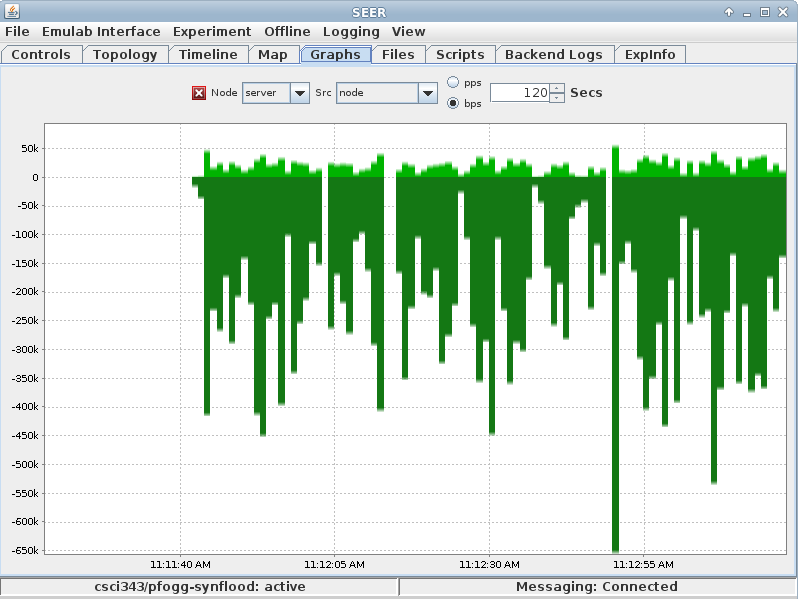
\includegraphics[width=3.5in]{green-traffic.png}
  \end{center}
\item The attacker is sending SYNs with a spoofed IP address, in order to look like the client. So the server's ACK messages are all going to the client, which looks like legitimate traffic.
  \begin{center}
    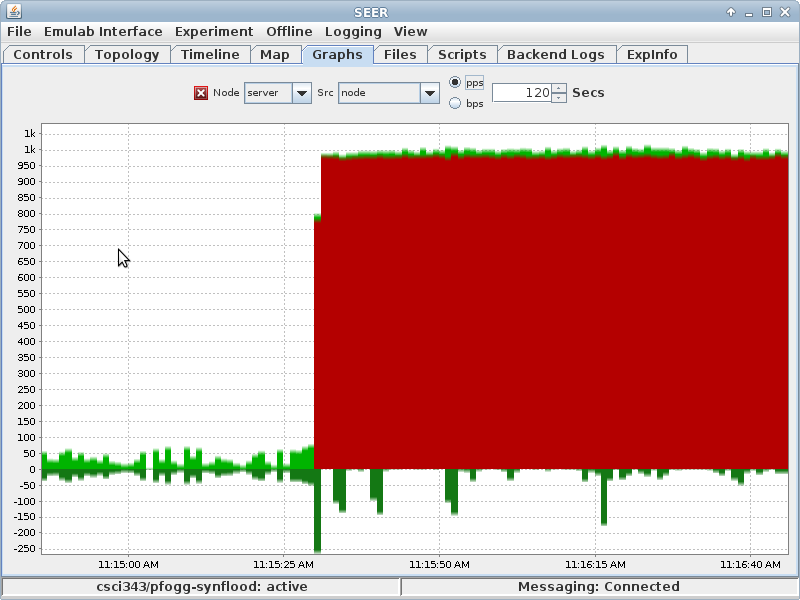
\includegraphics[width=3.5in]{red-traffic.png}
  \end{center}
\item \text{}
  \begin{center}
    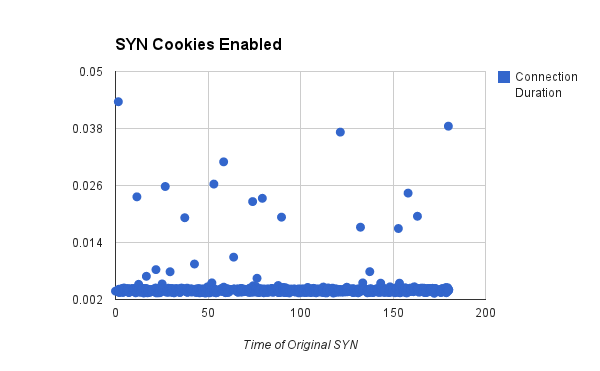
\includegraphics[width=3.5in]{with-cookies.png} \\
    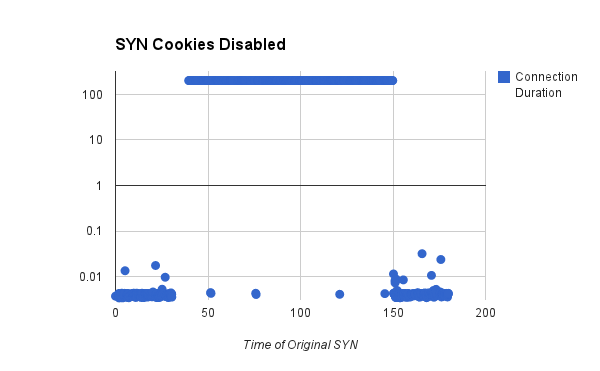
\includegraphics[width=3.5in]{without-cookies.png}
  \end{center}
\item
\item
\end{enumerate}
\end{document}
